
%\begin{abstract}
 
%\end{abstract}

%*****************************************
\chapter{Introduction and Motivation}
%*****************************************

% introduction
%	- general topic
%	- motivation (why is it necessary)
%	- problem statement (major issues, problem parts, %		proposed solution)
%	- overview of thesis structure
	
% general topic, motivation

With the ever increasing number of hard- and software systems that generate continuous streams of heterogeneous data it becomes more difficult to extract meaningful information from this data and act upon it in real time. \gls{cep} is a method that allows processing data streams from multiple sources by letting users specify events of interest as continuous queries. Events resulting from the combination of several simple and other complex events through aggregation, composition and derivation operators are called complex events.
If the \gls{cep} system detects a complex event that matches a query, all interested users will be notified of the event's occurrence immediately. 
If processing of the operators involved in detecting complex events is performed centrally on one computing node, scaling of the system in terms of joining data sources, additional queries or an increase of the data rate is obviously limited. 
Therefore, distributing the operators involved in the processing of the data over several computing nodes is beneficial, if not necessary, in many application scenarios.

Since applications that have to react in real time to occurring events require a certain \gls{qos} from the \gls{cep} engine, a solution to include \gls{qos} demands in a \gls{cep} system has been proposed with AdaptiveCEP \cite{Weisenburger2017a}.
It allows the specification of \gls{qos} demands on queries, e.g. that the end-to-end latency from data source over all participating processing nodes to the user has to be less than 100ms, or that the frequency of received events has to be above a certain rate. To satisfy such requirements, the choice of a fitting placement algorithm is crucial as it is responsible for the distribution of individual processing steps of a query onto a network of processing nodes. Every placement algorithm is designed with specific  assumptions about processing network characteristics (e.g. mobility, density) and \gls{qos} metric optimization goals in mind. These characteristics and the \gls{qos} demands from users constitute the context the system is operating in. Because of this, employing the wrong placement algorithm in a given context can have serious negative impact on the relevant \gls{qos} metrics and degrade performance of an application relying on the \gls{cep} system. 

\section{Problem Statement}
% problem statement (major issues, problem parts, proposed solution)
While in a static context only the initial choice of the placement algorithm is important, in an application scenario with dynamic context the optimal placement algorithm may change over time because the network conditions or \gls{qos} demands can change significantly, making a switch from one placement algorithm to another necessary. Such a change of mechanism is called a transition, triggered by the system moving from one context to another. The aspects that can be responsible for such a change are, among others, node topology (clustered vs. distributed) and traffic type (burst vs. uniform). 
% adaptation here refers to changes the system makes because of periodic recalculations to adapt to slight changes in network conditions;
% reconfiguration refers to changes in the adaptation strategy and its mechanisms (== adaptation on a higher level)
%TODO check for consistency with weisenburger paper, section 4B
%An adaptation strategy consists of several mechanisms (e.g. placement algorithm, query optimization) that determine how the system reacts to relatively small changes in the network \gls{qos} metrics.
The ability to dynamically reconfigure the mechanisms of the system at run-time based on the context is necessary to assure stable and reliable system operation in the face of significant changes in network conditions and user demands. 
In this work we will focus on reconfiguring the most influential mechanism, namely the deployed placement algorithm, but any other mechanism could be reconfigured as well. 

In order to perform reconfigurations of the mechanisms at run-time, we need two pieces of information: first, up-to-date information on the current context to determine if a significant environment change has occurred and what the new context is; and second the most fitting mechanism(s) to transit to in the new context.
 
%Context information is, according to Etzion: \textit{" [...] indirectly relevant information that is useful to functioning of the service, but not provided to the service as part of its invocation"}, so in our case, any information that is relevant for determining what mechanism to use (i.e. information about network conditions, network \gls{qos} metrics, \gls{qos} demands), but is not provided by the user as part of a query. 
%TODO source (Etzion paper)
%TODO problem: \gls{qos} demands are user-provided, but they are (very) relevant for determining what mechanism to use -> context or system in \gls{cfm}? more logical to keep it together with query \gls{qos} metrics

According to Dey \cite{Dey2001}, context is \textit{"any information that can be used to characterize the situation of an entity. An entity is a person, place, or object that is considered relevant to the interaction between a user and an application, including the user and application"}.
In our case, relevant information is any information that helps determining what mechanism to use (i.e. information about network conditions, network \gls{qos} metrics, user \gls{qos} demands) without the user having to set it manually.
This information must be captured in a structured way so that it can be automatically processed and used to determine the placement algorithm to be used.  
Due to the inherent variability of both system (utilized placement algorithm, processing nodes) and context we need a modeling technique that is suited to capture the possible configurations of our system and its context in a coherent way. 
Such a technique is available in the form of \glspl{dspl} which can be represented as graph-based \gls{fm}. Prior work has shown their ability to model context-based adaptation of a system with the help of so called \glspl{cfm} \cite{Saller2013} \cite{Acher2009}.
Feature Models can represent (Dynamic) Software Product Lines which model different variants of a software system. They are used to specify variation points and the possible alternatives (features) at these points as well as constraints between these alternatives. A product configuration is created by 
 selecting or deselecting every feature, and is only valid if it respects all constraints between features.
 
 As the several variable parts of the context are important for deciding what adaptation to make in the system, modeling them as separated System Features (directly configurable system parts, e.g. placement algorithm) and Context Features (influences that cannot be controlled directly, e.g. network metrics, \gls{qos} demands) together in one model is a reasonable choice.
 By interpreting different context states as different configurations, we can identify changes between contexts by observing changes in the configuration of the context side of the \gls{cfm} and then, based on these observations, trigger appropriate transitions from one mechanism to another, represented by a reconfiguration of the system side of the \gls{cfm}. 
 % reference to Saller paper, where reconfiguration of the system is handled by a transition system; number of possible reconfigurations is limited through constraints between context features and system features, which allows
 By structuring the model through constraints and dependencies (between context features and system features as well as among context features) the space of possible configurations is limited to valid ones. This limits the amount of possible reconfigurations of the system, in our case the choice of the placement algorithm, to those allowed by the model.  
 Our aim is to determine the most fitting placement algorithm for a given configuration of context features; to achieve this, we propose to either predict the performance of every placement algorithm that is allowed by the constraints in this context configuration through some form of regression, or train a classifier to predict the most fitting placement algorithm based on the current context. 
 %TODO to keep or not to keep?
 In the first case, model constraints limit the number of different placement algorithms to be considered for a given context; in the second case, the amount of required training data is limited to instances with valid context configurations.
 
 Automating the choice of a fitting placement algorithm would enable the system to adapt to known situations as well as new ones without the need for manual reconfiguration of the employed placement algorithm. \\ \\


% thesis goals/aims
\section{Goals}
This thesis aims to explore context-dependent transitions of mechanisms in \gls{cep} systems and how to model them in order to enable self-adaptation of the system's adaptation behaviour, specifically the placement algorithm. 
To achieve this, the following contributions will be made:
\begin{itemize}
\item Review of relevant literature on context modeling, especially with the help of feature models, and context-based adaptation of event-based systems
\item Identification of required properties of a context model to represent an adaptive \gls{cep} system
\item Design of a \gls{cfm} that allows to capture context changes and \gls{qos} demands. This model allows to restrict the space of valid mechanism configurations eligible for a transition
\item Design of a machine learning approach for placement algorithm selection based on user \gls{qos} demands and constraints imposed by the \gls{cfm}
\item To prove the applicability of our approach, the existing \gls{cep} system Adaptive\gls{cep} will be extended with a prototypical implementation of the designed context model and a module that allows adapting the deployed placement algorithm at run-time based on the context information gathered by our model
\item Evaluation of the implementation in selected simulated scenarios to quantify potential performance gains.
\end{itemize} 


% structure overview
%TODO adapt as necessary
\section{Outline}
The remainder of this document is structured as follows: 
chapter 2 includes background information on the topics of Complex Event Processing, Context Feature Models and Machine Learning and surveys and analyzes related work in the area of Context Feature Models in Dynamic Software Product Lines and adaptive \gls{cep} systems. Furthermore we will introduce an application scenario to give a practical example to refer to in the next chapters.
 In chapter 3 we will perform a context model requirement analysis for Adaptive\gls{cep}, present and justify our \gls{cfm} design and explain the prototypical implementation of the model and the adaptation mechanism.
 Chapter 4 covers the evaluation methods, results and their discussion
 In the final chapter 5 we will recap the thesis and reflect on the proposed solution and its results as well as possible future work.



\chapter{Background}
% general introduction into topics relevant to the thesis

% This chapter should give a comprehensive overview on the background necessary to understand the thesis. The chapter should have a length of about five pages!

\section{Event and Data Stream Processing}
% renamed, introduce DSP/ \gls{esp} (Data / Event Stream Processing), then explain relation to \gls{cep} (similarities and differences)   
% \gls{cep}: basics + relation to EBS and/or stream processing, placement algorithms, other mechanisms
% \gls{qos} metrics, importance of \gls{qos} demands  

% introduction to (Event) Stream Processing \\ \\

The task of processing streams of data produced by multiple sources has been approached from two different research directions. The first approach is inspired from the area of \glspl{dbms} which persistently store data and allow users to query it on demand. As this is not an applicable approach when dealing with applications that need to process continuous streams of data from from many sources and update the results of queries made to them by consumers in real-time, \glspl{dsms} have been developed to address this issue. \gls{dsms} allow users to apply SQL-like queries to potentially unbounded streams of data in a vein similar to \gls{dbms}. However, a major difference arises from the continuous nature of processed data: while in traditional \gls{dbms} a finite amount of data is stored persistently and can be accessed anytime, data streams are potentially unbounded and not persistent. This entails that instead of applying an incoming query to existing data, incoming data is applied to an existing query. Queries are treated as continuous (or standing) and update their results based on incoming data. They consist of common SQL operators like aggregations, select, join and all the operators defined in genral by relational algebra \cite{Cugola2012}. However, since \gls{dsms} usually do not support an ordering of arrived data, the detection of patterns in the processed data through operators like sequence is not possible.

The second approach is called \gls{cep} and views data streams as streams of events since it was developed in the context of event-based simulation \cite{Luckham}.
It can be seen as an extension to the content- and topic-based publish-subscribe paradigm \cite{Cugola2012}, as it allows subscriptions to refer not only to single events, but to events created through the combination of lower-level events from multiple heterogeneous sources.
%event definition
An \textit{event} can be defined as anything that happens \cite{Chandy2011}, or more precisely, any meaningful change of state in the universe of an application that can be perceived through some kind of (physical or virtual) sensor. Depending on the application, a mere change in time can be an event, so any ordered sequence of data generated by a source like a light sensor can be interpreted as an \textit{event stream}. To be precise, when we use the term \textit{event} we actually mean a \textit{notification about an event}, not the event itself that caused the change of state. This \textit{event notification} is a message that contains one or more attribute-value fields and usually has a time stamp and a type.

\gls{cep} allows more involved analysis of event streams since a time-stamped event model allows the events to be ordered, enabling sequence operators and pattern matching. This in turn makes the detection of causal relationships possible (if in a domain A causes B, a situation that is characterized by the occurrence of event A followed by event B can be detected)
%sequence operator, causal relationships
The of goal \gls{cep} is to extract higher-level information from a stream of lower-level events by declaratively specifying events of interest through event patterns, often expressed in a query language. This allows the timely detection of events representing situations of interest that demand a reaction. 

The processing of events with \gls{cep} can be summarized as follows: Data sources (producers) generate streams of simple events (e.g. sensor readings) which can be processed using operators that combine and correlate them with other events and domain knowledge to create complex events. Complex events in turn can serve as input for further operators. Interested parties (consumers) can subscribe to events of interest to them. These events of interest are represented by complex events and can be defined through queries consisting of aggregation, composition and derivation operators, which in turn are executed on event streams by the \gls{cep} system.

%types of operators in more detail \\
Queries - sometimes also referred to as event patterns \cite{Luckham2011a} or event definition rules \cite{Cugola2013} - consist of one or more operators connected in a graph. \gls{cep} operators can be categorized as follows \cite{Freudenreich2015}:
\begin{itemize}
\item Aggregation: operations that are applied to a finite set of values, like count, sum, average, median, minimum, maximum. Since streams are potentially unbounded, some form of windowing (tumbling or sliding window of the last x events or of the last y seconds) has to be applied to the stream so it can be processed by these operators.
\item Composition: combination of information from two or more events, not necessarily of the same type, into a new event. This event conveys new information by relating two or more events to each other. Typical composition operators include conjunction, sequence (specific events happen in order), negation of a sequence (a specific event does not occur between two events) \cite{Eckert2009}
\item Derivation: using knowledge about domain semantics and/or external knowledge, a new event is derived through reasoning about information from incoming events and information from knowledge
\end{itemize}

The event processing system is responsible for processing of incoming events and routing detected complex events to any interested consumers.
This allows for timely reaction to new information by the consumers, enabling a range of real-time, reactive applications.
%TODO possibly give example of Adaptive\gls{cep} query \\
%example
As an example, an event pattern correlates incoming 'Smoke Particle Detected' events from a smoke particle sensor with aggregated 'Temperature' events if the average temperature of the last 30 seconds exceeded 50 degrees Celsius. If the \gls{cep} system detects a series of events from sensors in close proximity to location X that matches this pattern, it creates a complex event 'Fire in location X detected' and emits it to the interested parties (e.g. building monitoring system). 

% short summary of possible applications \\
% applications (supply chain management, healthcare, transportation, manufacturing, financial trading) and their requirements, scaling issues (-> link to distributed processing)
\gls{cep} systems have various applications, among them the  domains of intrusion detection systems, credit card fraud detection, stock market trading, business intelligence, network monitoring, traffic monitoring, healthcare, transportation, supply chains and manufacturing. Due to the nature of some of these domains, event sources can be numerous and widely distributed and producing high amounts of data, making \gls{cep} systems that rely on central processing susceptible to scaling issues. This calls for a distributed computing approach, which exists in the form of Distributed \gls{cep}.
% explain relation to Data Stream Processing / Event processing 
% different origins of \gls{cep} and eps, terms converged over time; focus of \gls{esp}: bulk stream data processing, \gls{cep}: event pattern detection, causal dependencies -> find only the few relevant events in the stream
% distributed processing of cep and esp/dsms -> both relevant for thesis because operator placement is a problem for both
While \gls{dsms} systems rely mostly on aggregation operations to perform bulk data processing, \gls{cep} systems traditionally focus more on detecting temporal and causal correlations of particular events in order to abstract to a higher level of information \cite{Cugola2012}. Since both can be operated on a network of processing nodes, both need operator placement algorithms (which will be introduced in the next section) that are part of the mechanisms whose transitions are a focus in this work. Bearing the similarities in mind, both approaches are considered here since placement algorithms from the \gls{dsms} domain may be applicable in the \gls{cep} domain as well in certain application scenarios.
%focus on cep, but keep dsms in mind as well because of placement problem in distributed scenarios

%rename to dsp and placement algorithms
\subsection{Distributed Stream Processing and Operator Placement}
%queries, operator graphs
%clustered(cluster of highly connected hosts) vs networked/decentral
%placement algorithms \\
%purpose, assumptions, optimization goals, central vs decentral, task assignment problem NP-hard

While both \gls{dsms} and \gls{cep} systems can operate with a central processing unit, it is often beneficial to distribute the processing of data and event streams in order to increase efficiency, flexibility and scalability.   
The individual operators of an operator graph representing a query can be mapped to several independent, interconnected processing nodes (called hosts if an operator is deployed to them), forming an overlay network. Distributed processing makes \gls{cep} systems much more scalable and efficient: events do not incur additional producer-to-consumer latency from being routed to a central processing unit, network traffic is decreased because unnecessary events can be filtered on hosts closer to their sources, and operators can be replicated onto multiple hosts in case of high data rates and/or limited processing capabilities of hosts, allowing the system to scale in and out.

% terminology: placement algorithm/mechanism -> placement as an adaptation mechanism
%explanation of placement algorithms, goal, purpose, requirements
Operator placement algorithms are utilized to find and deploy a mapping of the queries submitted to a \gls{cep} system to the network of processing nodes which is optimal w.r.t. some non-functional property.
%NP-hard task assignment problem, heuristics
As the operator placement problem is a specific instance of the partition problem which has been shown to be NP-hard \cite{Cardellini2016}, placement algorithms find a placement that is close to the optimal one in reasonable time through heuristics that aim to optimize one or more \gls{qos} metric(s).
Optimizing a non-functional property such as latency is important e.g. in a scenario with geographically spread out producers and consumers where a certain end-to-end latency must not be exceeded. In this case it is not possible to route all events to a central processing node as it will likely cause the latency limit to be exceeded. Therefore the computations involved in processing a query must be distributed across nodes between producers and consumers that are connected via low-latency links and have short processing delay.
These non-functional properties and \gls{qos} metrics can be, among others: 
\begin{itemize}
\item end-to-end latency 
\item bandwidth consumption
\item CPU load (balancing)
\item reliability
\item availability
\item energy consumption
\end{itemize}
%TODO citations
Currently, most operator placement algorithms discussed in literature focus on optimizing latency \cite{Pandit2004} bandwidth \cite{Ahmad2004} \cite{Schilling2011}, load balancing \cite{Xing2005} or combinations of latency and bandwidth  \cite{Pietzuch2006} \cite{Rizou2010} or latency and load balancing \cite{Heinze2013}, but other metrics like energy consumption have been adressed as well \cite{Bonfils2004}. 
Besides optimizing one or more \gls{qos} metric(s), every placement algorithm is designed for specific situations characterised by network conditions like traffic type (bursty or uniform), network topology (distributed or clustered), and stability of connections and queries. 

%central vs decentral placement decisions
Placement algorithms can work in a centralized or distributed fashion, meaning that they have either information on the state of the entire network, allowing them to find globally optimal placements, or are restricted to local information from the node they are executed on and its neighbours, allowing them to make locally optimal placement decisions. Centralized algorithms tend to find globally better placements, but are restricted in their scalability due to the amount and frequency of necessary information exchange. 

%dependencies in operator graphs, other constraints
The placement of operators can be constrained: some operators may require a minimum of processing power or specific hardware; further constraints are imposed by sequential dependencies between operators: if an operator combines several simple or complex events, the operators that process these events need to be placed on processing nodes located upstream (viewed from the consumer) of this operator's processing node, so this can reduce the number of feasible solutions. 

Summarizing, for the calculation of an operator placement the following pieces of information are needed \cite{Lakshmanan2008}:
\begin{itemize}
\item the queries to be placed, viewed as logical flow graphs consisting of event sources, operators, and drains
\item the network of interconnected processing nodes that will host the operators of the flow graph
\item measures or estimates of non-functional properties of the network and its nodes that are decisive for the placement choices  to be made, including, among others, latency and bandwidth of links, availability, processing speed of operators on a node 
\item information about processing nodes' capabilities and operators' requirements that may constrain the placement
\end{itemize}


%other adaptation mechanisms
\subsection{Adaptation mechanisms in CEP}
%purpose of adaptation mechanisms
Since the environment a \gls{cep} system is operating in can vary, it needs mechanisms that let it adapt to different circumstances (contexts). The links of the network connecting the processing nodes as well as the state of nodes themselves may change; links may get congested or break down, nodes may fail or have changing load levels.
To account for this network context variability, operator placement algorithms of \gls{cep} systems compute the initial deployment of the operator graph onto its hosts based on measurements of non-functional properties gathered from the available processing nodes. 
To ensure that the placement remains optimal during run-time, an adaptation strategy may monitor changes in the \gls{qos} measurements and can periodically re-evaluate the current placement. It can then decide to adapt the placement through migration of single operators onto new hosts, though this might be limited to cases where expected performance gains exceed the estimated impact of the migration process to avoid constant oscillation of an operator between two hosts that would negatively affect performance.

% static placement algorithms -> motivation for thesis topic; adaptation of adaptation mechanisms
While periodic re-evaluation of the placement enables the system to react to changes in the underlying network to a certain degree, there is currently no way to automatically adapt the utilized placement algorithm or other mechanisms to major changes in the context that adversely affect the \gls{qos} demands of users. If any part of the network or application context (e.g. network conditions, network topology, type of \gls{qos} demands on queries, event frequency) is changed significantly, the adaptation mechanisms (e.g. placement algorithm) that was used before may no longer be optimal as it was intended for a different context. To guarantee a steady level of system performance and the observance of \gls{qos} demands imposed on the queries by users (if supported by the \gls{cep} system), some form of context awareness and adaptability of the system is necessary to make context-based transitions between different mechanisms possible.

%other mechanisms: query optimization, replication
Further mechanisms to keep \gls{qos} demands satisfied involve the optimization of the operator graph before its deployment to the network, as well as parallelization of processing steps by replication of the same operator onto multiple hosts to increase throughput (operator replication). It is also possible to identify parts of operator graphs that are identical for different queries and let several queries share these processing steps to avoid duplicate processing of events (operator re-use).

\section{Dynamic Software Product Lines and Feature Models}
% terms and definitions, FODA notation \\

%introduction: past(new software variant for every new product) -> near past SPLs and present DSPLs, re-use of modularized software, individual products derived from spl
With the complexity and size of software systems increasing over time, approaches have been envisioned that help reduce the time and effort necessary to develop a new software product. Often products similar to existing ones have to be developed that differ only in a small set of features and functions to fulfill customer-specific requirements.
\Glspl{spl} are used in Software Engineering to specify a family of software products that solve similar problems and as a consequence have a a set of commonalities and variation points. Instead of starting every product in an application domain from scratch, the parts of the software system that solve identical tasks within the domain can be re-used in individual products, saving development effort. 
\Glspl{spl} allow the systematic derivation of individual product variants based on the requirements imposed by a customer's application. 
% product configuration of an spl gained by binding all variability
An instance of a product from a product line is obtained by binding all variability captured in the \gls{spl} to a specific valid configuration of selected features.
% definition of feature (1 system property during domain engineering, 2 product configuration parameter during application engineering for deriving specific variants)
A feature can be defined as a relevant system property and is used to capture commonalities and variabilities among products in a product line \cite{Fernandes2008}; it is a distinctive user-visible system property identified during domain engineering and a product configuration parameter during application engineering \cite{Saller2013}.

%FMs
% FODA notation with an example (mock example of ...?), groups, constraints
%constraints -> model validation, valid configuration specification through FMs, restriction of valid configuration space
\textit{Feature models} are a formalism to represent a domain and the common and variable parts of a \gls{spl} in a tree structure and were first described in \cite{Kang1990}. They allow to define a hierarchical structure of alternative (xor, exactly one feature may be chosen), and-groups (all features are chosen) and or-groups (zero or more are chosen) of features. The choice of groups of features and individual features is either mandatory or optional. For a child feature to be selected, the parent must be selected as well, which allows the representation of hierarchical dependencies between features. Dependencies between features from different groups can be represented as cross-tree constraints in the form of the \textit{requires} (Fig.1, if Option A is selected Alternative A must be selected as well) and \textit{excludes} (Fig.1, Alternative A and Option B cannot be active at the same time) relations. Through the tree structure and the cross-tree constraints the space of valid feature configurations is confined to those that represent actually producible software products. Thus the feature model is a means to specify what products can be derived from the \gls{spl}.
It is possible to use constraint solvers to check the consistency of feature configurations of possible products.
%insert example graphic of a simple fm + explanation here
\begin{figure}
\centering
\caption{A simple Feature Model example}
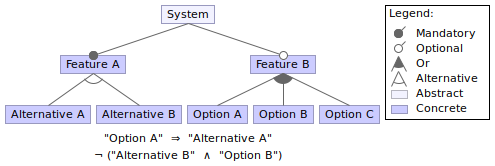
\includegraphics[scale=1]{FMexample.png}
\end{figure}

%TODO steps in dspl engineering: domain analysis (1. context analysis -> define bounds of the domain, 2. domain modeling -> describing the problems in the domain that are addressed, 3. architecture modeling -> create software architecture(s) that solve the problems), variation points, domain modeling (-> FM), architecture modeling
%To generate a feature model it is necessary to perform an analysis of the domain to be modeled (\textit{domain analysis}) in which every relevant system property is identified and mapped to a feature.
%feature analysis: 1. identify features 2. abstract and classify the features as a model (FM), defining the features 3. model validation
%The task of identifying and organizing commonalities and variabilities in the form of shared data and capabilities in a domain is called \textit{Domain Analysis} \cite{Kang1990}.

%dspls variability specified at design time
%runtime adaptability through dspls -> context information to trigger adaptations of the FM -> context-aware feature models CFMs, context-aware reconfiguration planning in saller2013
The more recent approach of \glspl{dspl} \cite{Hallsteinsen2008} allows to bind variability at run-time instead of development time, which can considerably improve a system's capabilities and performance since its configuration is adaptive instead of static during run-time. 
The concept of \glspl{dspl} offers a way to model transitions between different possible mechanisms in a system. This can be accomplished by modeling different mechanisms as features and representing transitions between mechanisms as reconfigurations in the system's feature model. Specifying transitions this way allows the amount of possible valid reconfigurations to be reduced, allowing the adaptation behaviour of a system to be modeled as transitions between configuration states.%connection to context-aware systems

\subsection{Context-Aware Feature Models} 
% relevance of context-awareness to enable adaptability of systems \\
% introduction to self-adaptive systems that profit from mechanism transitions, (examples in related work?)
\% may be moved to related work as it is best explained in context of other work and is directly relevant to the thesis
%"extension of dspl variability specification given by a context model with requirements imposed by the context environment"
%model system and context separately (acher)
% specify requirements of run-time contexts via cross-tree constraints between context and system -> provide preplanning and execution of product reconfigurations at runtime
It has been proposed \cite{Acher2009} \cite{Saller2013} \cite{Fernandes2008} to model system features and context features separately with the help of \glspl{dspl} to build context-aware systems. Context-aware systems are able to react to changes in their environment by monitoring the variable parts of their context, analyzing the changes, and then planning and executing an adaptation of their behaviour in a MAPE-, PCDA or similar control cycle. 
Modeling the context in features structured by a feature model along with the system itself allows the representation of both in a unified way; this makes it possible to represent context-based adaptation behaviour of the system through cross-tree constraints. Rules that decide what system features to select in the presence of specific context features can be expressed through \textit{requires and excludes} relations between the two feature categories. This allows the system to adapt itself to changing contexts at run-time by adjusting its feature configuration.


%\section{Machine Learning}
% depending on type of the actual technique used \\
% explanation of general principle, examples of application
%\subsection{Regression Learning}
%\subsection{Classification}



\chapter{Related Work}
\% relevant work on related topics \\
\% categorize, evaluate, summarize other works, show differences and parallels; similar solutions but not necessarily similar problems; understand limitations of other works -> avoid these limitations if possible)

\% This chapter should give a comprehensive overview on the related work done by other authors followed by an analysis why the existing related work is not capable of solving the problem described in the introduction. The chapter should have a length of about three to five pages!

\section{Context Modeling for Event-based Systems}

\subsection{Context Modeling Techniques}
\% survey related work on techniques that don't use FM, point out pros and cons \\
\% possible considerations for design and implementation, things to avoid and things to have \\ \\

%move this information to background?
Freudenreich explicitly differentiates between situation context (information about environment) and interpretation context (information about data). Regarding the modeling of situational context of event-based systems he identifies the following required features and characteristics, based on three surveys of different context models: 
\begin{itemize}
\item aspects:
\begin{itemize}
\item absolute and relative space and time 
\item application as subject
\item no context history or user profiles
\end{itemize}
\item representation: 
\begin{itemize}
\item key-value based
\item low formality
\item fully general, variable granularity
\item no valid context constraints
\end{itemize}
\item management: 
\begin{itemize}
\item context construction distributed and at runtime
\item basic context reasoning
\item hooks for incompleteness and context information quality monitoring
\item multi-context modeling
\end{itemize}
\end{itemize}
After identifying these requirements, he argues that there is a need for relationship representation and basic reasoning, but ontology-based models, which provide elaborate context reasoning, are considered to be too detrimental to EBS performance. Therefore he proposes an ontology-based metamodel that can represent domain con\gls{cep}ts in terms of con\gls{cep}ts, attributes and relationships which allows for context construction to happen at runtime, while the context information structure is determined at design time. The metamodel makes no assumptions about the domain model's data types or structure, making it very flexible. Situations and reactions to them can be specified declaratively as policies using the defined ontology.

E.Barrenchea et al. propose to embed context information directly into events as a first class element. Components can specify the context of their publications and/or subscriptions. Components can be grouped into contextual environments ( making them "siblings") that share the same context parameters and values. Context awareness is realized by context filters in an environment middleware layer that filter according to the specified event schema and the environment they are part of, which relieves components of keeping track of context information directly. This moves context away from the component logic and towards the layer of the pub/sub scheme.  An environment manager handles context updates and provides an interface to the application layer for utilizing  context information.

Koripip\"a\"a et al. present a software framework for context acquisition and processing in mobile scenarios. The API uses an extensible context ontology to define usable contexts. The context schema is defined in RDF syntax to ease the sharing of the ontology. Context has six possible properties: (first two are mandatory) 1. type 2. value 3. confidence 4. source 5. timestamp 6. attributes. It is possible to create context hierarchies and composite contexts.
The framework consists of a context manager (blackboard, delivers context information based on subscriptions), a resource server (collects and preprocesses context data from sources) and context recognition services (create higher-level contexts from atoms, can be plugged in at runtime). The recognition services make use of Naive Bayes classifiers and the confidence property to create higher-level contexts.

\subsection{Feature Models for Context-Aware Systems}
\% more detailed survey of Saller, Acher, Weckesser etc papers 

Some authors propose using feature models, which have their origins in the domain of highly configurable software product lines (SPL), as a means to model the variability and behaviour of context-aware systems.

M.Acher et al. \cite{Acher2009} suggest using two separate feature models: one for the system and its variable parts, and one for the context, each of them with its own constraints (e.g. require, exclude). This allows for a homogeneous representation of system and context and the relationships between the two. The two models are then linked together by dependency constraints which represent the adaptation behaviour. The adaptation of the system happens based on event-condition-action (ECA) rules, with elements of the context feature model as condition and a re-configuration of the system feature model as the action part. The authors mention optimization of a utility function as an alternative to ECA-rules for modeling adaptive behaviour, which would require the feature model to be extended with attributes for information needed for the optimization.

Saller et al. aim to enrich feature models with context information and context constraints in order to limit the set of valid configurations further. This is done to limit the complexity of re-configuration planning and enable such calculations on resource-constrained devices. Reconfiguration is modeled and pre-planned in the form of a transition system, with transitions from one valid system configuration into the next, based on context. To further reduce the amount of possible transitions, states with different configurations that satisfy the same constraints are considered to be identical in terms of transitions (incomplete state space). This model allows for multiple contexts to be active at once.

Weckesser et al. propose an approach that extends the expressiveness of feature models as well as the possibilities to validate them. It allows for modeling  of feature attribute types and constraints beyond boolean as well as UML-like multiplicities of features. Furthermore, they enable automated validation of such cardinality-based feature models through methods that check the constraints imposed on the feature model by cardinality annotations. This is useful when dealing with systems that have multiple instances of a feature and need to take dependencies among them (and their number) and other features into account.

\section{Adaptation and Context-Awareness for EBS}
\% Adaptive\gls{cep} paper\\ \\

%As some applications have specific requirements regarding the network conditions to function as intended, Adaptive\gls{cep} offers the possibility to include \gls{qos} demands with every query. These \gls{qos} demands, e.g. end-to-end latency < x or bandwidth > y, are used to ensure that every host between source and drain involved in the processing of a query helps satisfying these requirements. 

\% Lakshmanan placement algorithm classification \\
%TODO include relevant parts
The work of G. Lakshmanan et al. \cite{Lakshmanan2008} is a survey of 8 algorithms developed to solve the problem of optimal operator placement in data stream processing systems. To compare the different approaches, the authors define a set of core components that significantly affect the performance of the system and compare the categories of these components: 

\begin{itemize}
\item architecture (centralized, decentralized or hybrid implementation of placement logic)
\item algorithm structure (centralized vs decentralized decisions)
\item metric(s) to optimize (load, latency, bandwidth, machine resources, operator importance, combinations of those)
\item operator-level operations (reuse or replication of operators) 
\item reconfiguration (triggers for operator migration: thresholds, periodic re-evaluation, constraint violation)
\end{itemize}

Based on these components, 8 placement algorithms developed r\gls{esp}ectively by Pietzuch, Balazinska, Abadi, Zhou, Kumar, Ahmad, Amini and Pandit are assigned to the discussed categories. The authors then proceed by comparing the algorithms w.r.t. their design decisions and underlying assumptions. It is concluded that decentralized approaches which are able to adapt dynamically by operator migration are prevalent, with latency and, by extension, load balancing being the preferred metrics to optimize. 
Based on the comparison of the assumptions a decision tree for selecting a fitting placement algorithm considering the characteristics of a given problem (node distribution, number of administrative domains, dynamics of topology and data, query diversity) is proposed.


\section{Performance Prediction using Feature Models}
\% survey of SPLConqueror (if not used, replace section heading in accordance with other ML-related papers)

%TODO keep or remove?
SPLConqueror is a collection of programs and a library for discovering the influence of configuration options of software with variable elements on non-functional properties. This is done iteratively by using linear regression learning and stepwise feature selection. It consists of four programs: 
\begin{itemize}
\item VariabilityModelGUI: creation and editing of variability models of the configurable system; allows for exclude/require constraints between elements
\item Performan\gls{cep}redictionGUI: learning an influence model from a given variability model and a set of measurements (of configurations and their performance regarding one metric). Possible configuration options for sampling and linear regression algorithm are available. The result is a an influence model of terms of weighted influences on one specific performance metric in the following form: (w1*c1 + w2*c2 + ... w34*c3*c4) where w34*c3*c4 denotes the selection of both configuration options c3 and c4
\item SPLConquerorGUI: GUI for visualization and analysis of the learned model with options for filtering variables and adjustment of the model. Visualization of influences and detected dependencies
\item CommandLine: allows for specification and execution of experimental setups with different sampling and machine learning options
\end{itemize}
 Further submodules include MachineLearning (algorithm for learning performance-influence model; interface for SAT checking of configurations w.r.t variability model and optimization of configuration for a given non-functional property and objective function) and PyML (interface to scikitlearn (a python ML framework), different regression learning techniques).
 
 Application to Adaptive\gls{cep}: 
 1. determine from measurements for every mechanism (context (network conditions) -> performance (w.r.t. mechanism's optimized \gls{qos} metric?)) the influence of every context element on the performance metric by using linear regression; -> need to restrict combinations of context features + mechanisms to valid ones to limit necessary training/measurement data 
 2. the resulting formula (with weights for the influence of each context feature) can predict the performance of every context feature configuration for each mechanism 
 3. with this, calculate the predicted performance of every mechanism for a given context configuration
 4. compare the performance predictions of the different mechanisms for a given context configuration; problem: how to compare performance measured in different metrics? Can it be reasonably normalized to [0,1], if yes, what lower/upper bounds to choose for latency, bandwidth, ... to make them comparable?
 5. if reasonable comparison of performance metrics can be found: choose mechanism with best (normalised) performance for the given context
\section{Comparative Analysis and Discussion} 
\section{Summary}

\chapter{Context-aware Feature Model and Mechanism Transition Approach}

%Design
\% This chapter should describe the design of the own approach on a con\gls{cep}tional level without mentioning the implementation details. The section should have a length of about five pages
% 1. Requirements + Assumptions 2.System Overview 2.1 Component A, 2.2 ..., 3. Summary

\% in detail: problem analysis, identification of important issues, describe and explain proposed solution, identify remaining issues

%TODO old motivation, re-use?
%If an application has to be capable of adapting to changing conditions in its execution environment, it needs information on the aspects that can change over time and are relevant for adapting its behavior. This is achieved by representing the context of an application in a context model. According to Dey, context is \textit{"any information that can be used to characterize the situation of an entity. An entity is a person, place, or object that is considered relevant to the interaction between a user and an application, including the user and application"}. Other definitions of context exist, such as the following by Etzion: \textit{"Context is indirectly relevant information that is useful to functioning of the service, but not provided to the service as part of its invocation"}. Both definitions imply that context information has to be collected and stored in a way that enables the application to ensure it behaves according to expectations. As every application has different notions of what context information is to be considered relevant, the required features of a context model need to be identified based on the desired behavior of the application.


\section{Context Feature Model Design}
\subsection{Requirement Analysis}
In the case of Adaptive\gls{cep}, the system should be able to detect the conditions of the network that hosts the operators of its queries. In order to ensure the compliance with any \gls{qos} demands placed on the queries, it should then be able to dynamically choose appropriate mechanisms (operator placement strategy, ...) that fulfill the demands and optimize their relevant \gls{qos} metrics even if the network conditions change. 
To do this, the application needs knowledge about the status of any nodes currently hosting operators (to detect performance deterioration) as well as alternative nodes currently unoccupied (for possible reconfiguration).
Some of this information could be abstracted into coarser categories to facilitate decision making.
Furthermore, it should be able to cope with joining and leaving hosts. 
The adaptability of the application is given by the different strategies therefore it should be possible to include new strategies, possibly with new types of \gls{qos} metrics. Useful dimensions of network status information are, among others: latency, bandwidth, utilization, throughput, location/velocity (in case of mobile network entities), energy consumption.

%Context Model Requirements
To capture the requirements of the context model in a structured manner, the analysis framework proposed by Bolchini et al. is used. This categorizes the requirements as follows: \\
1. Modeled Aspects \\
\newline
\begin{tabularx}{\textwidth}{|X|X|}
\hline
\textbf{Feature} & \textbf{Analysis Result} \\
\hline 
space & yes, necessary for proximity demands \\ 
\hline 
time & maybe, for "freshness" of information \\ 
\hline 
absolute/relative space and time (coordinates/timestamp vs. near/after something)  & abs.+relative space, absolute time \\ 
\hline 
context history (does the current context state depend on previous ones)  & unclear, maybe for stability metrics of links; needed for machine learning purposes? \\ 
\hline 
subject (what is the point of view -> user or app perspective) & app centric, system needs context information to optimize strategy usage \\ 
\hline 
user profiles (are user preferences relevant for the context, how are they represented) & \gls{qos} demands can be viewed as user preferences \\ 
\hline 
\end{tabularx} 


2. Representation Features \\
\newline
\begin{tabularx}{\textwidth}{|X|X|}
\hline
\textbf{Feature} & \textbf{Analysis Result} \\
\hline 
type of formalism (key-value, markup, logic, graph, ontology -> different intuitiveness, reasoning possibilities)  & Context Feature Model == graph-based, logic for constraints \\ 
\hline 
flexibility (domain specific vs general)  & specific to application, with enough flexibility for extensions \\ 
\hline 
variable context granularity (ability to represent context at different levels of detail) & - \\ 
\hline 
valid context constraints (can the number of possible contexts be restricted by semantic constraints) & necessary to restrict space of system configurations; inherent to \gls{cfm} \\ 
\hline 
\end{tabularx} 
 
 3. Context Management and Usage \\
\newline
\begin{tabularx}{\textwidth}{|X|X|}
\hline
\textbf{Feature} & \textbf{Analysis Result} \\
\hline 
context construction (central description of possible contexts at design time vs distributed construction of the current context at runtime) &  central description of context dimensions, distributed construction by collection of current values \\ 
\hline 
context reasoning (ability to infer properties or construct higher-order context information from sensor readings) & maybe, abstract from measurements to situations \\ 
\hline 
multi-context modeling (one instance of the model can represent all possible context, not one instance for each context) & yes, need to model changes between contexts \\ 
\hline 
\end{tabularx} 

\subsection{Context-aware Feature Model Proposal}
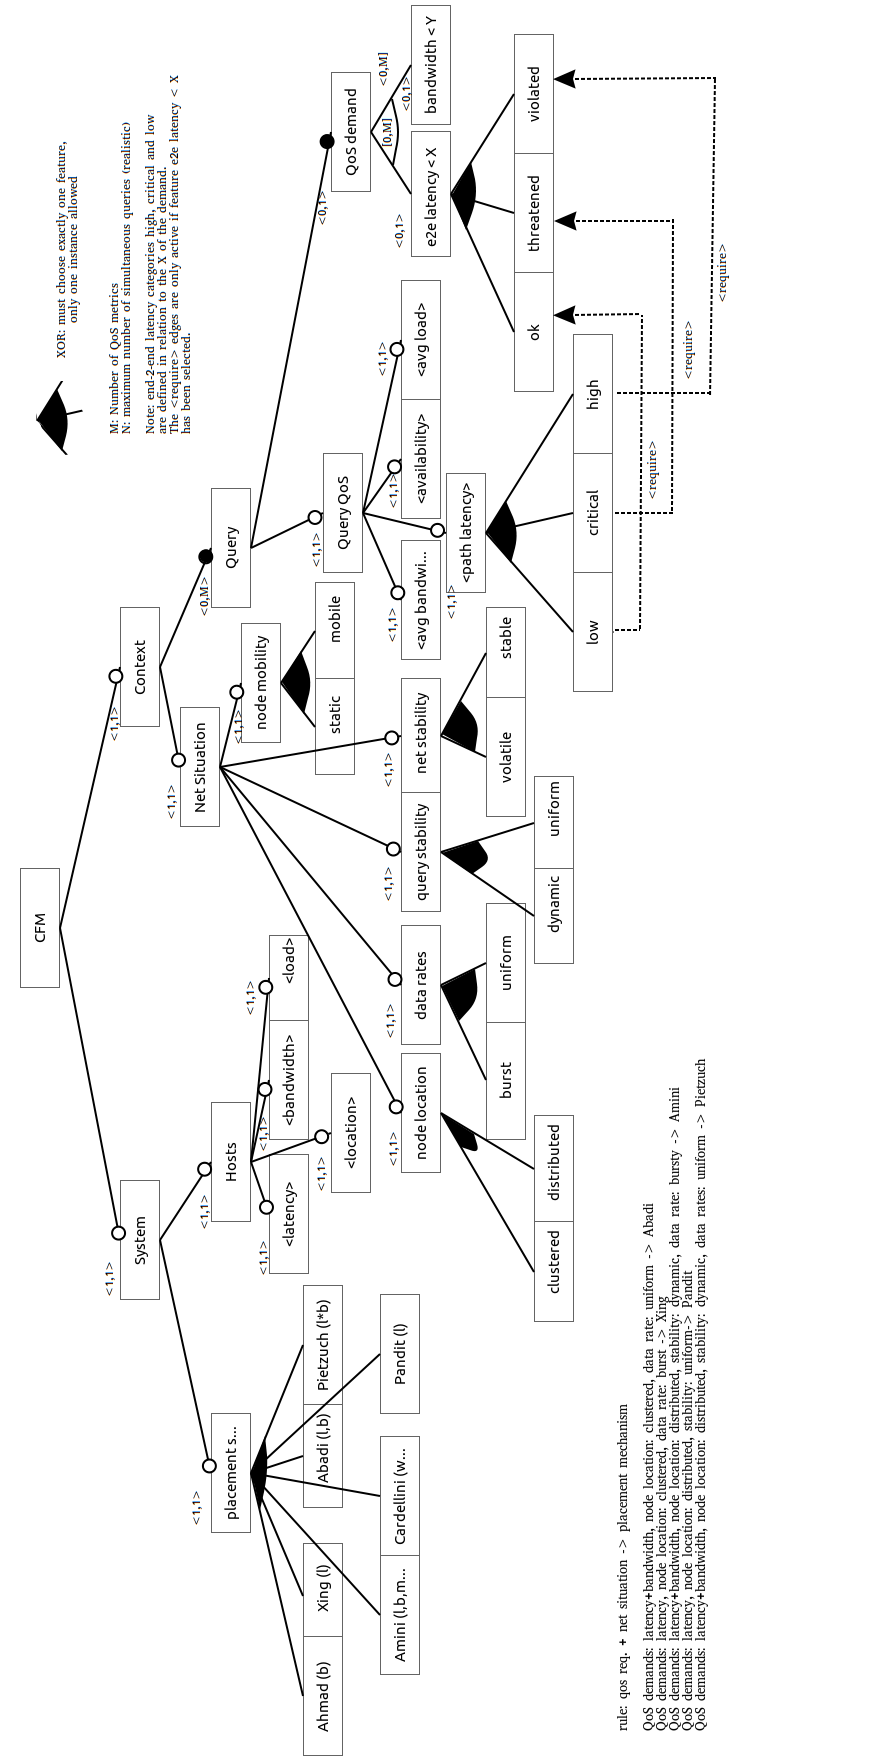
\includegraphics[scale=0.4]{alternative3.png}

Note: will split graph in system and context part for better readability 


The model limits itself to those elements of the system that are relevant for the detection of or reaction to network environment changes.
The graph modeling technique used to represent the context model as a feature model was first used in the domain of Software Product Lines (SPL) and allows definition of variable parts (features) of both system and context. At runtime, the active features constitute the configuration of the system/context; the space of possible configurations is restricted by constraints between features (xor-, or groups, require- and exclude relations). This allows the restriction of the model to valid configurations, which is helpful when gathering measurement data for different possible configurations. 
The main elements of the context are the queries executed by the system, their \gls{qos} metrics, the \gls{qos} demands placed upon them, and a set of situations that characterize the network conditions of the nodes in the system. These situations abstract from measurements on single hosts to the overall state of the queries' environment, and can be used in the definition of constraints and adaptation rules. Their mutually exclusive subcategories (like dynamic, uniform) can be defined by threshold values (in some relation to \gls{qos} demands on operators) and can be defined more finely granular if necessary. Note that multiple Situations can be active at the same time.
The variable parts of the System are the ones that can be directly reconfigured: the placement mechanisms, each optimizing a set of \gls{qos} metrics and suited to a certain situation. Although they can not be directly reconfigured, the Hosts/Nodes are an integral part of the system, so they are included on this side of the model. Every Host in the System has a set of associated \gls{qos} measurements.
For the sake of readability, constraints among the features of the model can as well be noted separately as follows: 
\newline
\begin{center}
 (C1) Situation:data rate:burst \textbf{and} Situation:node location:clustered \textbf{and} Query:\gls{qos} demand: e2e latency < X \textbf{requires} placement:Xing\\
 
 \end{center} 
with Xing being a placement strategy that aims to minimize the latency.
Adaptations from one strategy to another could be triggered in a similar manner:

\begin{center}
(A1) Query:\gls{qos} demand:latency \textbf{and} Query \gls{qos}:path latency:high \textbf{implies} other latency optimizing strategy\\

\end{center}

\section{Mechanism Transition Prediction Approach}
\section{Summary}

\chapter{Implementation}
% Implementation
\% This chapter should describe the details of the implementation addressing the following questions:
\%1. What are the design decisions made?
\%2. What is the environment the approach is developed in?
\%3. How are components mapped to classes of the source code?
\%4. How do the components interact with each other?
\%5. What are limitations of the implementation?
\%The section should have a length of about five pages.

% 1. Design Decsisions 2. Architecture 3. Interaction of Components 4. Summary

Preliminary Implementation Considerations:
\begin{itemize}
\item context information could be distributed via context events; a context manager subscribes to context sources and the application (or adaptation strategy) subscribes to the aggregated events from the context manager
\item context source monitoring could happen similar to the existing MonitorFactories
\item create a new interface for the context elements (metrics, attributes, constraints) and its management
\end{itemize}


\section{Design Decisions}
\section{Architecture}
\subsection{Context Feature Model}
\subsection{Mechanism Transition Prediction Approach}

\section{Interaction of Components}
\section{Summary}


\%This chapter should describe how the evaluation of the implemented mechanism was done.
\%1. Which evaluation method is used and why? Simulations, prototype?
\%2. What is the goal of the evaluation? Comparison? Proof of con\gls{cep}t?
\%3. Wich metrics are used for characterizing the performance, costs, fairness, and efficiency of the system?
\%4. What are the parameter settings used in the evaluation and why? If possible always justify why a certain threshold has been chose for a particular parameter.
\%5. What is the outcome of the evaluation?
\%The section should have a length of about five to ten pages
% 1. goal and methodology 2. setup 3. resutls 4. analysis
\chapter{Evaluation}
\section{Methodology}
\% describe how performance is measured

\section{Evaluation Setup}
\% describe testenvironment setup
\% describe test cases for transitions between mechanisms triggered by context changes

\section{Results}
\% compare system performance in test cases with and without context awareness (if there are implementation variants, compare these as well)
\section{Analysis and Discussion}
\% does the solution improve performance, what issues are there and why


\chapter{Conclusion}

\%This chapter should summarize the thesis and describe the main contributions of the thesis.
\%Subsequently, it should describe possible future work in the context of the thesis. What are limitations of the developed solutions? Which things can be improved? The section should have a length of about three pages.
%1. Summary 2. Contributions 3. Future Work 4. Final Remarks
\% brief recap of work so far, discuss findings of analysis -> what are strengths and shortcomings of the solution, new problems -> future work

\section{Summary}
\section{Contributions}
\section{Future Work and Final Remarks}


%*****************************************
%*****************************************
%*****************************************
%*****************************************
%*****************************************